\documentclass{beamer}
\usepackage[latin1]{inputenc}
\usepackage{graphicx}
\usepackage{hyperref}
\usepackage[font=small,skip=0pt]{caption}

\usetheme{Warsaw}
\title[Neural LM]{Exploring the Limits of Language Model}
\author{Raghavendra R Bilgi}
% \institute{Math-linux.com}
\date{Feb 21, 2017}
\begin{document}

\begin{frame}
\titlepage
\end{frame}


\begin{frame}{Automatic Speech Recognition (ASR)}
	\begin{itemize}
		\item Main component of Voice Assistants
		\item Converts Speech to text (STT)
		\item Goal is to recognize as many words correctly as possible (low Word Error Rate (WER))
	\end{itemize}

	\begin{block}{Fundamental Equation of Speech Recognition}
			\begin{align*}
				W^{*} =& \underset{W}{argmax}\ p(W/O; \Theta) \\
				W^{*} =& \underset{W}{argmax}\ p(O/W; {\Theta}_A)\ p(W; {\Theta}_{L})
			\end{align*}
	\end{block}
\end{frame}


\begin{frame}{Language Model (LM)}
	\begin{itemize}
		\item $P(O/W)$ links state sequence to words
		\item $P(W)$ Assigns Probability (prior) on word sequences
	\end{itemize}

	\begin{align*}
		P(W) =&\ P(w_1,w_2,w_3,...,w_N) \\
		     =&\ \prod_{n=1}^{N}\quad p(w_n/w_1,w_2,...,w_{n-1})
	\end{align*}

	\begin{itemize}
		\item Use n-gram models
		\item Probability is conditioned on window of n previous words
	\end{itemize}

	\begin{align*}
		Unigram  :&\ P(w_n)   \\
		Bigram   :&\ p(w_n/w_{n-1})  \\
		Trigram  :&\ p(w_n/w_{n-2}, w_{n-1})
	\end{align*}
\end{frame}


\begin{frame}{Language Model (LM)}
	Advantages of n-gram language models

	\begin{itemize}
		\item Performance improvement with higher n-gram (more context)
		\item Faster score computation (Faster look up)
		\item Can be represed as a WFST (useful for speech) 
		% \item [Remove] cannot be compiled into an FST, it has the wrong structure for that. You cannot obtain lattices with RNNLM scores directly but you can rescore them. Decoding Graph.
		\item Can be easily adpated to specific domain
	\end{itemize}

	Limitations

	\begin{itemize}
		\item Data spartisity is an issue
		\item More data, Smoothing, interpolation, back-off's required
		\item Exponential increase in the size with n-gram, and requrie more RAM
	\end{itemize}

% 	Scalable Modified Kneser-Ney Language Model Estimation
\end{frame}


\begin{frame}{Language Model in ASR}
	\begin{itemize}
		\item Two pass decoding stratergy used
		\item Smaller LM to generate the lattice which can fit in GPU memory
		\item Unpruned (bigger lm) to rescore the lattice
		\item Selection of pruning and smoothing method and stratergy is critical
		\item Agressive LM pruning has effect with certain smoothing techniques
		\item Lower Beam can result in shallow lattice
	\end{itemize}
\end{frame}


\begin{frame}{Language Model in ASR}
	Variants of Language Model

	\begin{itemize}
		\item Class n-gram model
		\item Cache model
		\item Skip-Gram Model
		\item Maximum entropy model
	\end{itemize}	
\end{frame}


\begin{frame}{Amazon Echo Study and Findings}
	\begin{figure}
	   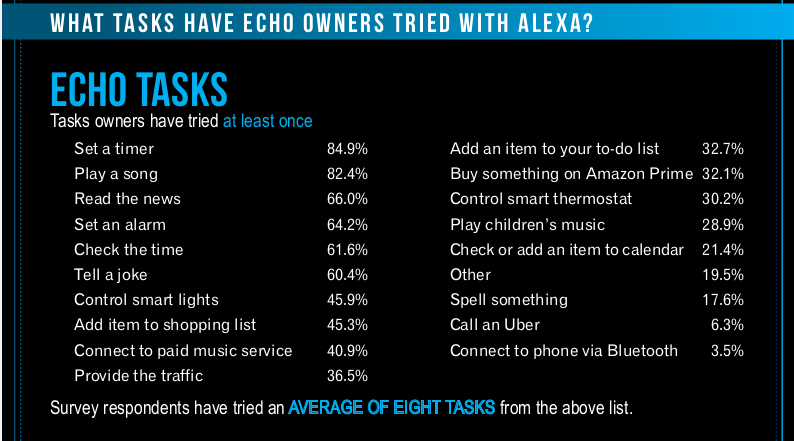
\includegraphics[width=11cm, height=6cm]{figs/echo_tasks.png}
	\end{figure}

	\href{https://www.experian.com/innovation/thought-leadership/amazon-echo-consumer-survey.jsp}{Source : Amazon Echo Study and Findings}
\end{frame}


\begin{frame}{Alexa Voice Shopping}
	\begin{figure}
	   
\includegraphics[width=11cm, height=6cm]{figs/alexa_deals_1.png}
	\end{figure}

	\href{https://www.amazon.com/b?node=14552177011}{Source : Alexa Voice Shopping}
\end{frame}


\begin{frame}{Alexa Voice Shopping}
	\begin{figure}
	   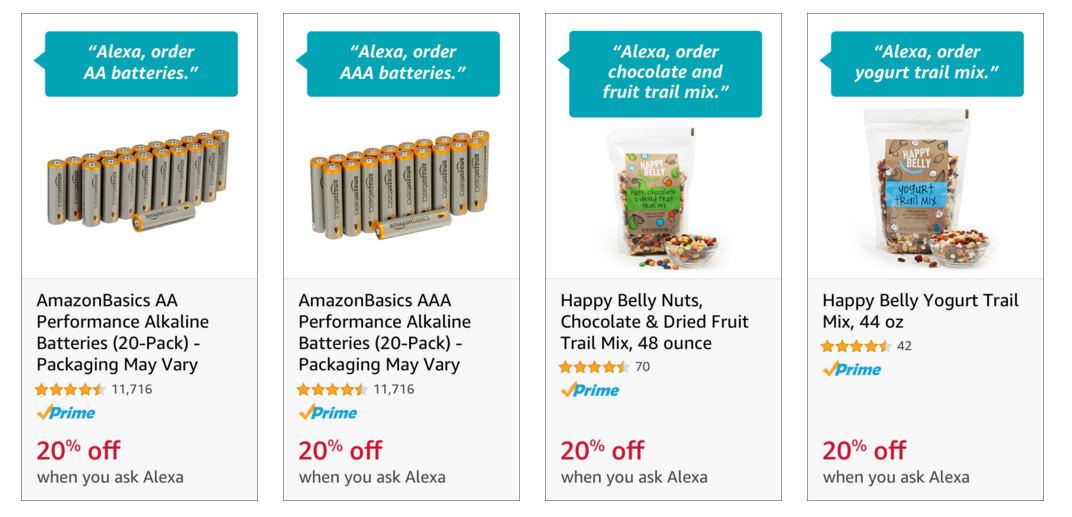
\includegraphics[width=11cm, height=6cm]{figs/alexa_deals_2.png}
	\end{figure}

	\href{https://www.amazon.com/b?node=14552177011}{Source : Alexa Voice Shopping}
\end{frame}


\begin{frame}{Alexa Voice Shopping}
	\begin{figure}
	   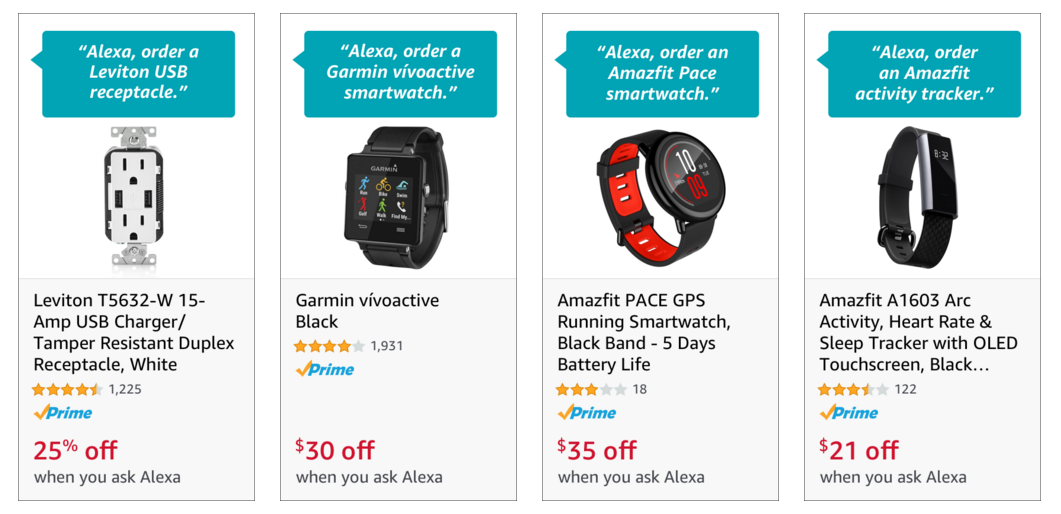
\includegraphics[width=11cm, height=6cm]{figs/alexa_deals_3.png}
	\end{figure}
	\href{https://www.amazon.com/b?node=14552177011}{Source : Alexa Voice Shopping}
\end{frame}


\begin{frame}{Google Voice Shopping}
	\begin{figure}
	   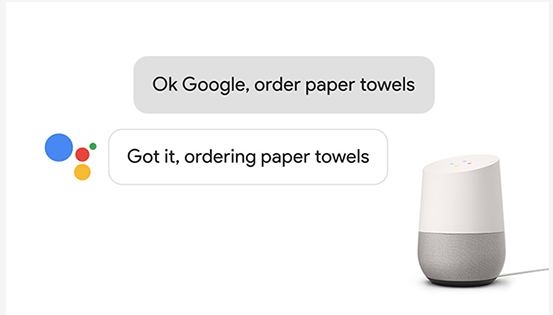
\includegraphics[width=11cm, height=6cm]{figs/googlehome_voiceshopping.png}
	\end{figure}
	\href{https://blog.google/products/home/start-shopping-google-assistant-google-home/?}{Source : Shopping with Google Assistant, Feb 16, 2017}
\end{frame}


%\begin{frame}{Alexa Voice Shopping}
%	\begin{figure}
%	   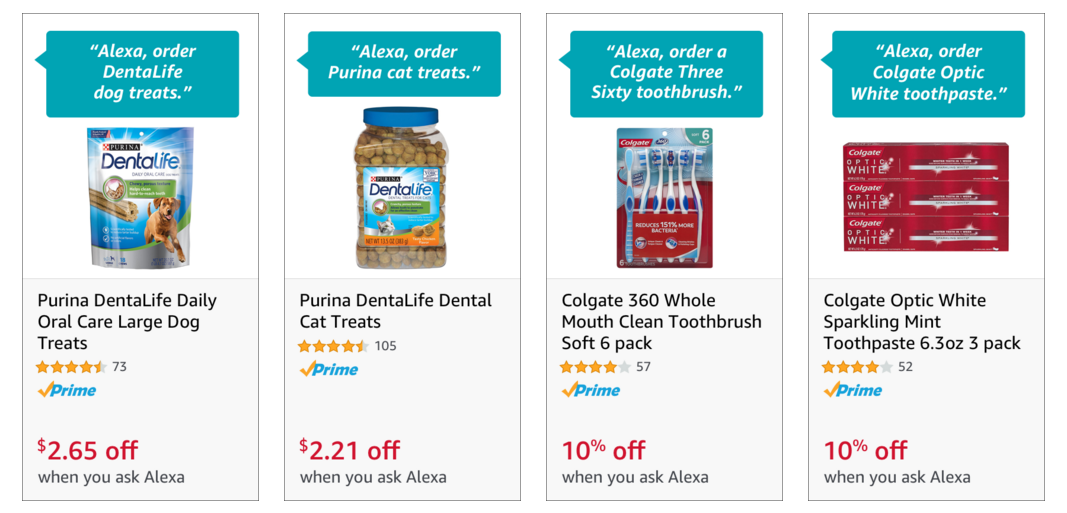
\includegraphics[width=11cm, height=6cm]{figs/alexa_deals_4.png}
%	\end{figure}
%
%	\href{https://www.amazon.com/b?node=14552177011}{Source : Alexa Voice Shopping}
%\end{frame}

%\begin{frame}
%	\begin{figure}
%	   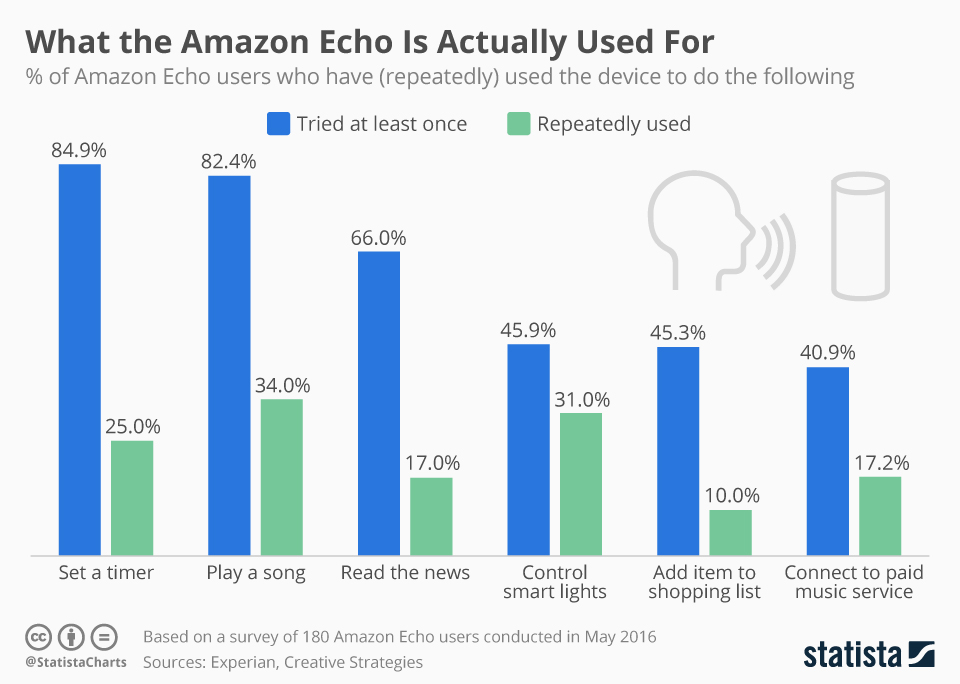
\includegraphics[width=11cm, height=8cm]{figs/chartoftheday_6080_amazon_echo_usage_n.jpg}
%	\end{figure}
%\end{frame}


\begin{frame}{Alexa Voice Shopping}
	\begin{block}{Amcrest IP2M-841 1080p dome surveillance camera}
		\begin{itemize}
			\item Wifi security camera black
			\item Amcrest i. p. to m. security camera
			\item wifi dome surveillance
			\item Amcrest indoor don't surveillance camera
			\item Amcrest dumb surveillance camera
			\item Amcrest ip to him surveillance camera
			\item Echo crest eight four one security camera
			\item Amcrest ten eighty p wi fi security camera
		\end{itemize}
	\end{block}

	\href{https://www.cnet.com/news/why-i-wanted-to-strangle-my-amazon-echo-on-prime-day/}{Source : Amazon Echo Prime day Review}
\end{frame}


\begin{frame}{Alexa Voice Shopping}
	\begin{block}{Amcrest IP2M-841 1080p dome surveillance camera}
		\begin{itemize}
			\item Amcrest IP2M security camera $\to$ Amcrest i. p. to m. security camera
			\item Amcrest IP2M surveillance camera $\to$ Amcrest ip to him surveillance camera
			\item Amcrest 841 security camera $\to$ Echo crest eight four one security camera
			\item Amcrest dome surveillance camera $\to$ Amcrest dumb surveillance camera
			\item Amcrest 1080p wi-fi security camera $\to$ Amcrest ten eighty p wi fi security camera
		\end{itemize}
	\end{block}

	\href{https://www.cnet.com/news/why-i-wanted-to-strangle-my-amazon-echo-on-prime-day/}{Source : Amazon Echo Prime day Review}
\end{frame}


\begin{frame}{Alexa Voice Shopping}
	\begin{block}{Noisy LM Training data}
		Kanvas Katha Women's Multi color Ballet Flats - 3 UK/India (36 EU)(KKFTOXDOCT00303) \\
		Royal Son Rimless Rectangular Women Spectacle Frame (RS0650ER 50 Transparent) \\
		Syska B22 15-Watt LED Bulb (Pack of 2, Cool Day Light) \\
		\underline{FabHomeDecor} Elzada Five Seater Sofa 3+2 (Black) \\
		Goodway Pack Of 3 Junior Boys Graphic Tee C'mon Bro-Give Your- Lazy Boy Prints Combo \\
		Butterflies Women's Wallet (Dark Pink) (BNS 2320 DPK) \\
		Fila Unisex Relaxer III Red and Navy Sneakers - 7 UK/India (41 EU) \\
		\underline{Vvoguish} Full Sleeve Indigo Red Round Size -S-VVTOP928INDGMELRD-S \\
		Skil 6513 JD 13mm Drill Kit with 15 Drill Bits \\
		IDEE Round Sunglasses (IDS1986C2SG 49 Matte Black)
	\end{block}

	\href{www.amazon.in}{Source : Amazon GIS Product List}
\end{frame}


\begin{frame}{Recurrent Neural Network Language Model (RNN LM)}
	\begin{itemize}
		\item Recurrence allows for unbounded context
		\item RNN Model compactly represents world knowledge
		\item Impressive Perplexity improvemnts
		\item No more feature engineering, model learns to extract latent features
	\end{itemize}

	\begin{figure}
	   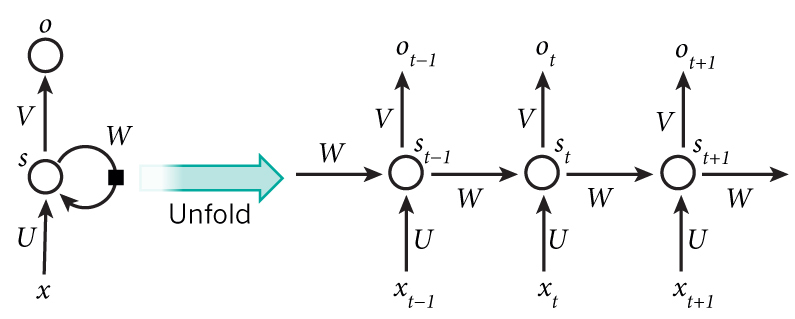
\includegraphics[width=11cm, height=4cm]{figs/rnn_unfloding.jpg}
	   \caption{A recurrent neural network and the unfolding in time of the computation involved in its forward computation : Source Nature}
	\end{figure}
\end{frame}


% ptb_rnnlm_mikolov_2011.png
% Extensions	of	recurrent	neural	network	language	model	by	Mikolov	et	al	2011

\begin{frame}{RNN LM}
	\begin{align*}
		h_{t} =&\ f(W_{t}h_{t-1}\ + U_{t}x_{t}) \\
		y_{t} =&\ softmax(h_{t}V_{t}) \\
		% y_{t} is probability distribution over all words
		% Same	cross	entropy	loss	function	but	predicting	words	instead	of	classes
		% p(y_1,y_2,...,y_{T'}/x_1,x_2,...,x_T) =&\ \prod_{t=1}^{T'}\quad p(y_t/h_{t}, y_1,...,y_{t-1})
	\end{align*}

	% The last hidden state summarizes the entire source sentence.
	\begin{figure}
	   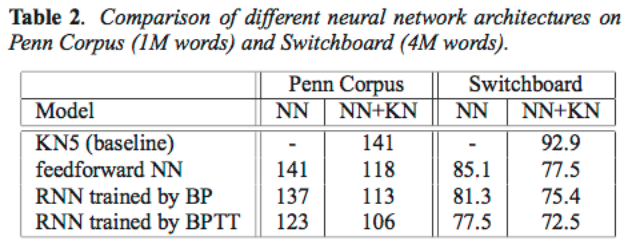
\includegraphics[width=10cm, height=4cm]{figs/ptb_rnnlm_mikolov_2011.png}
	   \caption{RNN LM Perplexity [Mikolov et al. 2010]}
	\end{figure}
\end{frame}


\begin{frame}{Distributional Representation of Words}
	\begin{itemize}
		\item Word meaning defined in terms of vectors
		\item Vectors are learned such that, words with similar context are close in vector space
		\item CBOW, Skip-Gram to learn the parameters
	\end{itemize}


	\begin{figure}
	   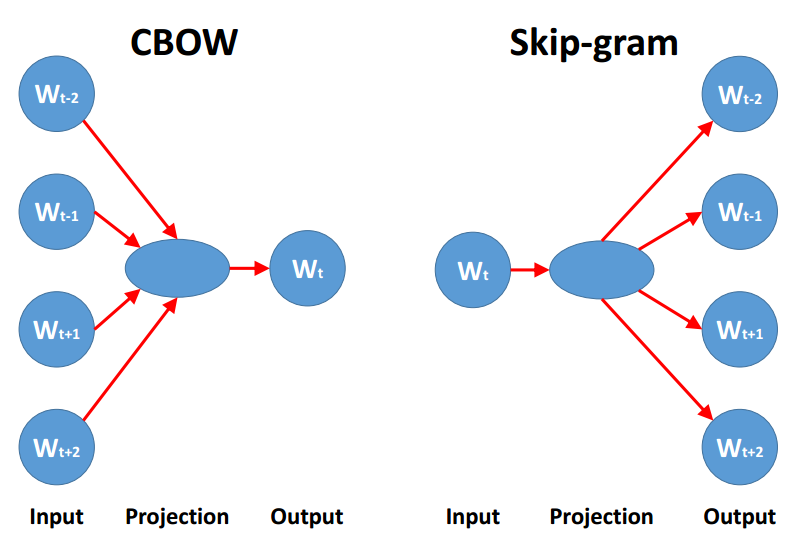
\includegraphics[width=7cm, height=5cm]{figs/cbow_and_skipgram.png}
	   \caption{CBOW and Skip-Gram Models}
	\end{figure}
\end{frame}


\begin{frame}{Sequence to Sequence model}
	\begin{align*}
		h_{t} =&\ f(W_{t}h_{t-1}\ + U_{t}x_{t}) \\
		y_{t} =&\ softmax(h_{t}V_{t}) \\
		% y_{t} is probability distribution over all words
		% Same	cross	entropy	loss	function	but	predicting	words	instead	of	classes
		p(y_1,y_2,...,y_{T'}/x_1,x_2,...,x_T) =&\ \prod_{t=1}^{T'}\quad p(y_t/h_{t}, y_1,...,y_{t-1})
	\end{align*}

	% The last hidden state summarizes the entire source sentence.
	\begin{figure}
	   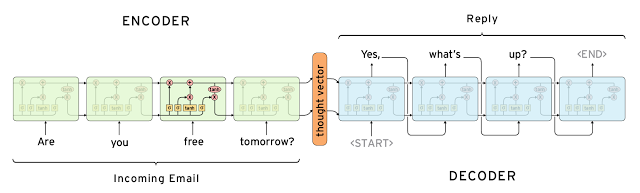
\includegraphics[width=11cm, height=4cm]{figs/encoder_decoder_rnn.png}
	   \caption{Sequence to Sequence Model}
	\end{figure}
\end{frame}



\begin{frame}{Sequence to Sequence model with Attention}
	% The last hidden state summarizes the entire source sentence.
	\vspace*{-2mm}	

	\begin{figure}
	   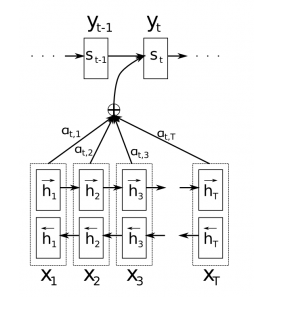
\includegraphics[width=5cm, height=4cm]{figs/seq_to_seq_with_attention.png}
	   \caption{Sequence to Sequence Model with Attention}
	\end{figure}

	\vspace*{-10mm}

	\begin{align*}
		c_{i} =& \sum_{j=1}^{T_x}\alpha_{ij}h_{j} \\
		\alpha_{ij} =& \frac{\exp(e_{ij})}{\sum_{k=1}^{T_x} \exp(e_{ik})} \\
		e_{ij} =&\ a(s_{i-1}, h_j)
	\end{align*}


%Here, The y‘s are our translated words produced by the decoder, and the x‘s are our source sentence words. The above illustration uses a bidirectional recurrent network, but that’s not important and you can just ignore the inverse direction. The important part is that each decoder output word y_t now depends on a weighted combination of all the input states, not just the last state. The a‘s are weights that define in how much of each input state should be considered for each output. So, if a_{3,2} is a large number, this would mean that the decoder pays a lot of attention to the second state in the source sentence while producing the third word of the target sentence. The a's are typically normalized to sum to 1 (so they are a distribution over the input states).

	\href{https://arxiv.org/pdf/1409.0473.pdf}{\tiny Source : Neural Machine Translation by jointly learning to align and transalate}
\end{frame}


%\begin{frame}{Recurrent Neural Network Language Model (RNN LM)}
%	Recent distributional real-valued representations
%	of words (examples: word2vec, GloVe)
%	have transformed the landscape of NLP applications
%
%	The success
%	comes from the geometry of the representations
%	that efficiently captures linguistic regularities: the
%	semantic similarity of words are well captured by
%	the similarity of the corresponding vector representations;
%	the latent relation between two words
%	is well captured by the difference vector between
%	the corresponding two vector representations.
%\end{frame}
%
%
%\begin{frame}{Recurrent Neural Network Language Model (RNN LM)}
%	Classic n-gram models of language cope with rare and unseen sequences by using smoothing methods,
%	such as interpolation or absolute discounting (Chen \& Goodman, 1996). Neural network models,
%	however, have no notion of discrete counts, and instead use distributed representations to combat
%	the curse of dimensionality (Bengio et al., 2003). Despite the effectiveness of distributed representations,
%	overfitting due to data sparsity remains an issue. Existing regularization methods, however,
%	are typically applied to weights or hidden units within the network (Srivastava et al., 2014; Le et al.,
%	2015) instead of directly considering the input data.
%
%	The technique of randomly zero-masking input word embeddings for learning sentence representations
%	has been proposed by Iyyer et al. (2015), Kumar et al. (2015), and Dai \& Le (2015), and
%	adopted by others such as Bowman et al. (2015). However, to the best of our knowledge, no analysis
%	has been provided besides reasoning that zeroing embeddings may result in a model ensembling
%	effect similar to that in standard dropout. This analysis is applicable to classification tasks involving
%	sum-of-embeddings or bag-of-words models, but does not capture sequence-level effects. Bengio
%	et al. (2015) also make an empirical observation that the method of randomly replacing words with
%	fixed probability with a draw from the uniform distribution improved performance slightly for an
%	image captioning task; however, they do not examine why performance improved.
%\end{frame}


\begin{frame}{RNN LM with CNN Softmax}
	\vspace*{-2mm}

	\begin{figure}
	   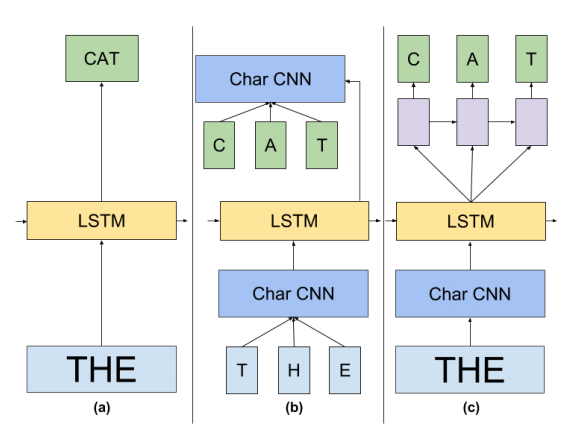
\includegraphics[width=5cm, height=4cm]{figs/exploring_limits_of_lm.png}
	\end{figure}

	\vspace*{-5mm}

	\begin{figure}
	   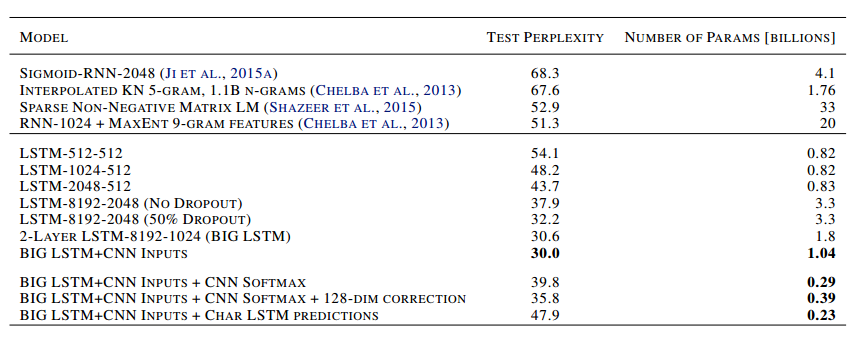
\includegraphics[width=8cm, height=4cm]{figs/results_exploring1.png}
	   \caption{Exploring Limits of Language Model, [Jozefowiez et al. 2016]}
	\end{figure}
\end{frame}


\begin{frame}{Neural Cache Model}
	\vspace*{-2mm}

	\begin{figure}
	   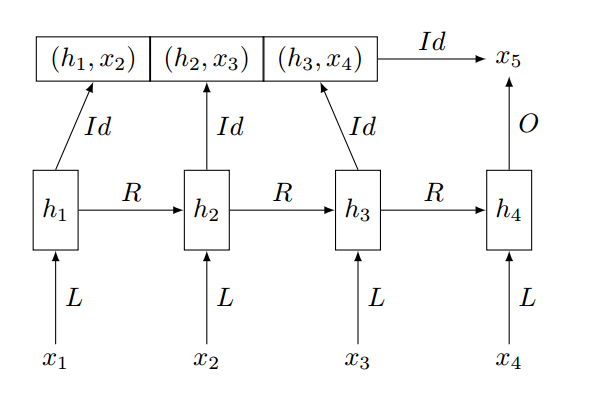
\includegraphics[width=5cm, height=4cm]{figs/neural_cache_lm.png}
	\end{figure}

	\vspace*{-5mm}

	\begin{figure}
	   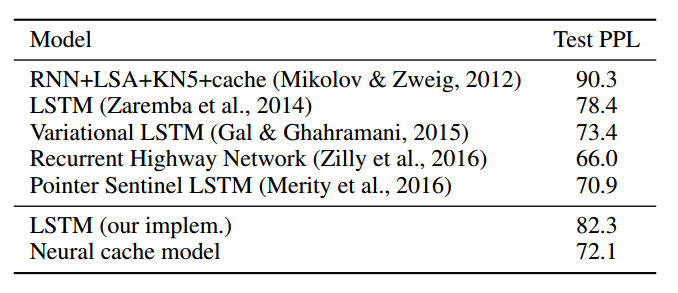
\includegraphics[width=8cm, height=4cm]{figs/neural_cache_model_ptb.png}
	   \caption{Neural LM with Continuous Cache, [Edouard Grave et al. 2017]}
	\end{figure}
\end{frame}


\begin{frame}{Ensemble of Language Model}
	\begin{figure}
	   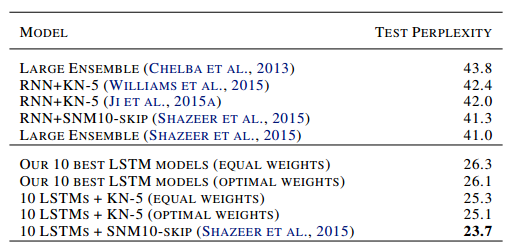
\includegraphics[width=7cm, height=5cm]{figs/results_exploring_lm2.png}
	   \caption{Ensemble of LM, [Jozefowiez et al. 2016]}
	\end{figure}
\end{frame}


\begin{frame}{N-Gram LM or RNN LM}
	\begin{itemize}
		\item RNN LMs are very popular results in lower perplexity
		\item However, they are not easy to adapt, cannot scale to to several million word dataset like n-grams
		\item RNN LM can't be compiled into an FST but can rescore the word lattice.
		\item Primary domains of Voice-Assistants use short utterances
		\item Ensemble of these to seems to be best middle gound
		\item n-gram model with context or domain knowledge is much better than single model
	\end{itemize}
\end{frame}


\begin{frame}
	\begin{figure}
	   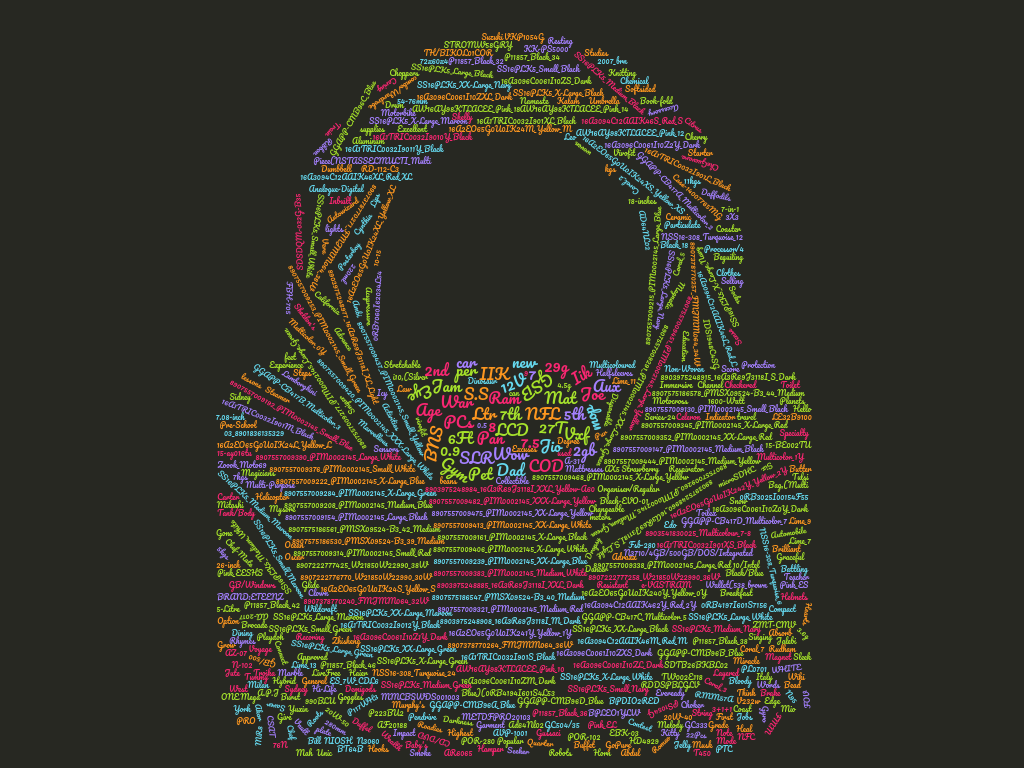
\includegraphics[width=11cm, height=8cm]{figs/word_cloud_gis_2.png}
	\end{figure}
\end{frame}


\begin{frame}
	\begin{figure}
	   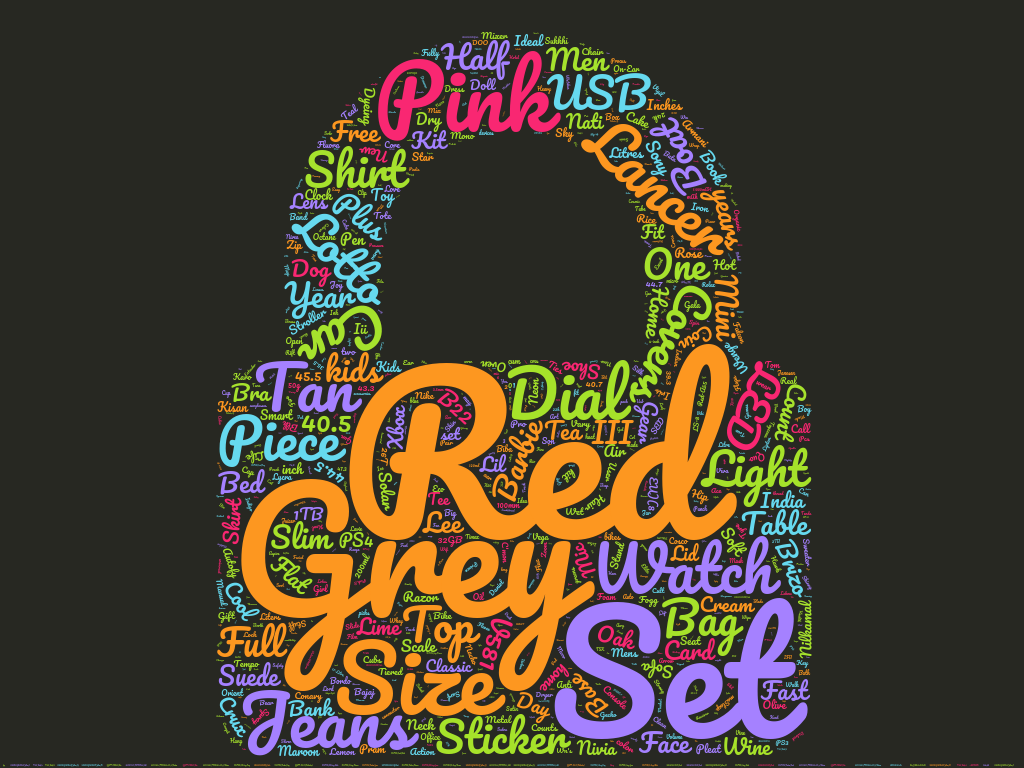
\includegraphics[width=11cm, height=8cm]{figs/word_cloud_gis.png}
	\end{figure}
\end{frame}


\begin{frame}{N-Gram LM or RNN LM}
	\begin{itemize}
		\item RNN LMs are very popular results in lower perplexity
		\item However, they are not easy to adapt, cannot scale to to several million word dataset like n-grams
		\item Primary domains of Voice-Assistants use short utterances
		\item Ensemble of these to seems to be best middle gound
		\item n-gram model with context or domain knowledge is much better than single model
		\item Lot of domain specific clean data
	\end{itemize}
\end{frame}



\end{document}
